\documentclass{article}

\usepackage{listings}
\usepackage{color}
\usepackage{courier}
\usepackage{amsmath}
\usepackage{graphicx}
\usepackage{float}
\usepackage[spanish]{babel}
\usepackage[utf8]{inputenc}
\usepackage{mleftright}
\usepackage{amsfonts}
\usepackage{hyperref}
\usepackage{csvsimple}
\usepackage{geometry}
\usepackage{esdiff}
\usepackage{array}

%% comandos sacados de stackexchange

% fuente: https://tex.stackexchange.com/questions/188775/how-to-type-a-particular-kind-of-unit-vector
\newcommand{\uvec}[1]{\boldsymbol{\hat{\textbf{#1}}}}

% fuente: https://tex.stackexchange.com/a/685485
\newenvironment{system}%
{\left\lbrace\begin{array}{@{}l@{}}}%
	{\end{array}\right.}

% fuente: https://tex.stackexchange.com/a/314612
\newcommand{\lnn}[1]{%
	\ln\left(#1\right)%
}
\newcommand{\lnb}[1]{%
	\ln\mleft(#1\mright)%
}


\title{PEC VI - Física Computacional II}
\date{07-01-2024}
\author{Arturo Felipe Albacete Fernández}



\lstset{
	basicstyle=\footnotesize\ttfamily,
	breaklines=true,
	frame=tb,
	tabsize=4,
	columns=fixed,
	showstringspaces=false,
	showtabs=false,
	keepspaces,
	commentstyle=\color{red},
	keywordstyle=\color{blue}
}
\lstset{frame=single}


\begin{document}

% titulo
\maketitle
\newpage

% TOC
\tableofcontents
\newpage

% intro
%
% Introducción
%

\section{Introducción}

\paragraph{}
En este documento se encuentran redactadas las respuestas a la Prueba de Evaluación Continua 3. Se ha utilizado Python como lenguaje de programación y LaTeX para generar este documento.

\subsection{Sobre este documento}

\subparagraph{Estructura}
A cada pregunta se le ha dedicado una sección, en la que se intenta responder a los distintos puntos de la cuestión así como una explicación del código relacionado a la solución de dicha pregunta. En algunos casos, si una pregunta ya ha sido contestada en un apartado anterior, lo anotaré. 

\subparagraph{Código}
El código para esta (y otras PECs) lo estaré publicando en un repositorio git. Se puede acceder via:

\begin{lstlisting}[language=bash]
	git clone https://gitlab.com/aalbacetef/fisica-comp-II.git entrega-aalbacetef-fc-ii
\end{lstlisting}


Si se desea, puedo enviar por correo electrónico el código del proyecto en archivo comprimido (tar/rar/zip/7z/etc...).

Gran parte del código lo he puesto en el apéndice, pero recomiendo ver el repositorio git para poder leerlo más cómodamente.


\subsection{Ejecutar el código}

Para ejecutar el código es necesario tener Python instalado. He facilitado esto con el uso de Docker y un Makefile. Las instrucciones de como ejecutar se pueden encontrar en el README.md del repositorio.

\subsection{Información de contacto}

Si necesita contactarme por alguna razón, aparte de mi correo electrónico de la UNED, puede contactarme mediante:
\begin{itemize}
	\item \textbf{Email:} aalbacetef@gmail.com
\end{itemize}

\subsection{Afirmación de autoría del trabajo}

\paragraph{}

El firmante de este trabajo reconoce que todo él es original, de su única autoría, escritura
y redacción, y que allí donde han sido empleadas ideas o datos de otros autores, su
trabajo ha sido reconocido y ubicado, con suficiente detalle, como para que el lector
pueda consultar lo afirmado sobre él.
\newpage

\section{Ejercicio A - La segunda ley de Newton}

\subsection{Problema}

Plantee la segunda ley de Newton para la partícula cuando el campo eléctrico y magnético son ambos uniformes, constantes y perpendiculares entre sí. Simplifique para el caso particular $\vec{E} = (0, 1, 0) \frac{V}{m}$, $\vec{B} = (0, 0, 1)\ T$.

\subsection{Análisis}

La segunda ley de Newton define la fuerza sobre un cuerpo como:

\begin{equation}\label{eq:1}
	\vec{F} = m \vec{a}
\end{equation}
La fuerza de Lorentz sobre una partícula de masa $m$ y carga $q$ es:

\begin{equation}
	\vec{F} = q(\vec{E} + \vec{v} \times \vec{B})
\end{equation}

\subsection{Resolución}



En el caso de que $\vec{E} = (0, 1, 0) \frac{V}{m}$, $\vec{B} = (0, 0, 1)\ T$:

\begin{align*}
\vec{F}(t)  
& =
	q(\uvec{j} + \vec{v}(t) \times \uvec{k}) \\
& =
	q(\uvec{j} + v_y \uvec{i} - v_x \uvec{j} ) \\
& = 
	qv_y \uvec{i} + q(1-v_x)\uvec{j} \\
& =
	q \begin{bmatrix}
		v_y \\
		1 - v_x \\
		0
	\end{bmatrix}
\end{align*}

Igualando esto con \eqref{eq:1}, nos da:

\begin{equation*}
	q \begin{bmatrix}
	v_y \\
	1 - v_x \\
	0
\end{bmatrix} = m \vec{a}(t)
\end{equation*}
\newpage


\section{Ejercicio B - Sistema de EDO}

\subsection{Problema}

Obtenga el sistema de ecuaciones diferenciales ordinarias de primer orden que es matemáticamente equivalente al sistema de ecuaciones diferenciales obtenido en el apartado anterior.

\subsection{Análisis}

La aceleración $\vec{a}$ también se puede escribir como:

\begin{equation}
	\vec{a}(t) = \diff{\vec{v}(t)}{t}
\end{equation}

\subsection{Resolución}

Tomando el resultado anterior:

$$
	q \begin{bmatrix}
	v_y \\
	1 - v_x \\
	0
\end{bmatrix} = m \vec{a}(t)
$$

Podemos reescribir $\vec{a}(t)$ como:

$$
\begin{bmatrix} a_x \\ a_y \\ a_z \end{bmatrix} =
\begin{bmatrix} 
	\diff{v_x}{t} \\ \\
	\diff{v_y}{t} \\ \\
	\diff{v_z}{t} 
\end{bmatrix}
$$

Esto nos da la siguiente ecuación:

$$
q \begin{bmatrix}
	v_y \\
	1 - v_x \\
	0
\end{bmatrix} = m \begin{bmatrix} 
\diff{v_x}{t} \\ \\
\diff{v_y}{t} \\ \\
\diff{v_z}{t} 
\end{bmatrix}
$$

y el sistema de ecuaciones (usaré $\dot{f}(t) = \diff{f(t)}{t}$ para ser conciso):
\begin{align*}
	q v_y - m \dot{v_x} &= 0 \\
	q(1 - v_x) - m \dot{v_y} &= 0 \\
	-m \dot{v_z} &= 0
\end{align*}
	
\newpage

\section{Ejercicio C - Como aplicar el método RK4}

\subsection{Problema}

Describa detalladamente como aplicar el método de Runge-Kutta de orden cuatro al sistema de ecuaciones diferenciales ordinarias del apartado previo. En concreto, obtenga explícitamente las expresiones funcionales de los coeficientes de Runge-Kutta implicados en la resolución.

\subsection{Análisis}

El método de Runge-Kutta de orden 4, en un contexto vectorial, está definido para un problema de valor inicial:

$$
\diff{\vec{y}}{t} = \vec{f}(t, \vec{y})
$$

con $\vec{y}(t_0) = \vec{y_0}$. 

Así que lo primero es replantear el sistema del apartado anterior: 


\begin{align*}
	q v_y - m \dot{v_x} &= 0 \\
	q(1 - v_x) - m \dot{v_y} &= 0 \\
	-m \dot{v_z} &= 0
\end{align*}

para que tenga la misma forma. Podemos reajustar y tener:

\begin{align*}
	\dot{v_x} &= \frac{q}{m} v_y \\
	\dot{v_y} &= \frac{q}{m}(1 - v_x) \\
	\dot{v_z} &= 0
\end{align*}

Lo cual da que:

$$
\vec{y}(t) = \vec{v}(t)
$$

\begin{equation}\label{eq:vel_deriv}
\vec{f}(t, \vec{v}) = \frac{q}{m} \begin{bmatrix}
\vec{v}(t) \cdot \uvec{j} \\ \\
1-\vec{v}(t) \cdot \uvec{i}\end{bmatrix}
\end{equation}

donde he usado el producto-punto en vez de $v_x(t)$ y $v_y(t)$ para ser explícito.

\newpage 

\subsection{Resolución}

El algoritmo de Runge-Kutta de orden 4 se trata, de forma general, en computar cuatro coeficienties $\vec{k}_i$, y usarlos para aproximar $\vec{y}$.

Los 4 coeficientes son, por $i = 0 ... n$.

\begin{align*}
	\vec{k}_1 &=
h\vec{f}(t_i, \vec{y}_i) \\
	\vec{k}_2 &=
h\vec{f}(
	t_i + \frac{h}{2}, 
	\vec{y}_i + \frac{\vec{k_1}}{2}
) \\
	\vec{k}_3 &=
h\vec{f}(
	t_i + \frac{h}{2}, 
	\vec{y}_i + \frac{\vec{k}_2}{2}
) \\
	\vec{k}_4 &= 
h\vec{f}(
	t_i + h,
	\vec{y}_i + \vec{k}_3
)
\end{align*}

y en cada paso: 

\begin{align*}
	t_{i+1} &= t_i + h \\
	\vec{y}_{i+1} &=
\vec{y}_i + \frac{1}{6}(
	\vec{k}_1 +
	2\vec{k}_2 +
	2\vec{k}_3 +
	\vec{k}_4
)
\end{align*}

\paragraph{Expandir el sistema} Para resolver por $\vec{r}(t)$ y $\vec{v}(t)$ a la vez, expandimos el sistema de la siguiente manera.

Primero definimos un vector $\vec{w}(t) = [\vec{r}(t); \vec{v}(t)]$:

\begin{equation*}
	\vec{w}(t) = 
\begin{bmatrix}
	r_x(t) \\ r_y(t) \\ r_z(t) \\
	v_x(t) \\ v_y(t) \\ v_z(t)
\end{bmatrix} = 
\begin{bmatrix}
	\vec{r}(t) \\ \vec{v}(t)
\end{bmatrix}
\end{equation*}

y su derivada es:

\begin{equation*}
	\diff{\vec{w}(t)}{t} =
\begin{bmatrix}
	\diff{\vec{r}(t)}{t} \\ \\
	\diff{\vec{v}(t)}{t}
\end{bmatrix} =
\begin{bmatrix}
	\vec{v}(t) \\
	\vec{f}(t, \vec{v}(t))
\end{bmatrix}
\end{equation*}

donde $\vec{f}(t, \vec{v}(t))$ es la que hemos definido en \eqref{eq:vel_deriv}.


\paragraph{Código} El código que implementa el método RK4 se puede ver en \ref{code:rk4}.
\newpage

\section{D - RK4 para un electrón}

\subsection{Problema}

Sea la partícula un electrón, es decir, con carga $q = -1.602 \cdot 10^{-19} C$  y masa $m = 9.109 \cdot 10^{-31} kg$. Realice la resolución numérica del problema con el método de Runge-Kutta de orden cuatro para los tiempos $t \in [0 \text{s}, 2\cdot10^{-10} \text{s} ]$ utilizando un paso de tiempo $\Delta t = 1 \cdot 10^{-12} \text{s}$ y con las condiciones iniciales de la posición $r(t = 0) = (0, 0, 0) \text{m}$ y velocidad inicial $v(t=0) = (0, 1, 0) \frac{\text{m}}{\text{s}}$.  Indique los resultados obtenidos para todas las magnitudes (posiciones y velocidades de la partícula) calculadas con el Runge-Kutta en las dos primeras iteraciones temporales.

\subsection{Resolución}

El código que resuelve el ejercicio se puede ver en \ref{code:ex4}.

Los resultados completos se pueden ver en el repositorio git y los primeros 50 puntos están en \ref{data:r_v_nonrel}. 

Los valores para las dos iteraciones temporales son:


\begin{table}[H]
	\centering
	\csvreader[
	tabular=|c|l|l|l|,
table head=\hline \textbf{t} & \textbf{$r_x$} & \textbf{$r_y$} & \textbf{$r_z$} \\\hline,
	filter test=\ifnumless{\thecsvrow}{3},
	late after last line=\\\hline,
	]{data/simul_no_rel_r.csv}{}{\csvlinetotablerow}
\end{table}

\begin{table}[H]
	\centering
	\csvreader[
	tabular=|c|l|l|l|,
	table head=\hline \textbf{t} & \textbf{$v_x$} & \textbf{$v_y$} & \textbf{$v_z$} \\ \hline,
	filter test=\ifnumless{\thecsvrow}{3},
	late after last line=\\\hline,
	]{data/simul_no_rel_v.csv}{}{\csvlinetotablerow}
\end{table}



\newpage

\section{Ejercicio E - Gráficas}

\subsection{Problema}

Represente en una misma gráfica $x(t)$, $y(t)$, $z(t)$ en función del tiempo. Represente $x(t)$ en función de $y(t)$. A la vista de los resultados, ¿quéconclusiones puede extraer sobre el movimiento de la partícula? Sin necesidad de ajustes, obtenga una estimación de la velocidad de arrastre de la partícula (también llamada de deriva) y de la frecuencia ciclotrón. Compare con los valores teóricos esperados.


\subsection{Resolución}

El código que resuelve este ejercicio se puede ver en \ref{code:ex5}.

\paragraph{Gráficas de los componentes de $\vec{r}(t)$}

A continuación está la gráfica de los componentes del vector de posición en función del tiempo.

\begin{figure}[H]
	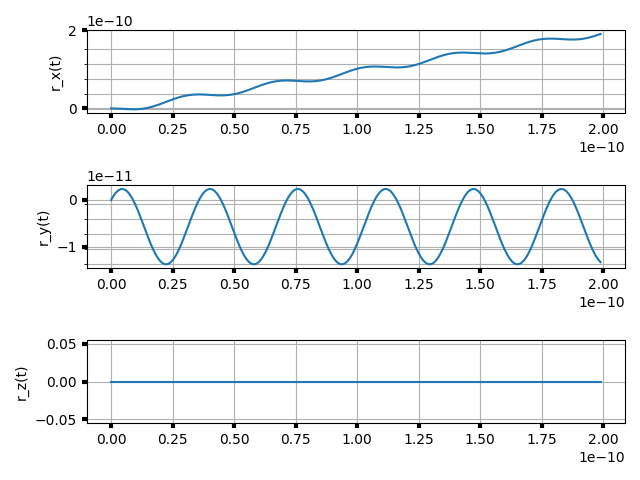
\includegraphics[width=\linewidth]{figures/no_rel_rx_ry_rz.png}
	\caption{Gráfica $r_x(t)$, $r_y(t)$, $r_z(t)$ en función de $t$}
	\label{fig:no_rel_x_y_z_t}
\end{figure}

\newpage 

\paragraph{Gráficas de $\vec{r}_x(t)$ y $\vec{r}_y(t)$}

A continuación está la gráfica de $r_x(t)$ en función de $r_y(t)$.

\begin{figure}[H]
	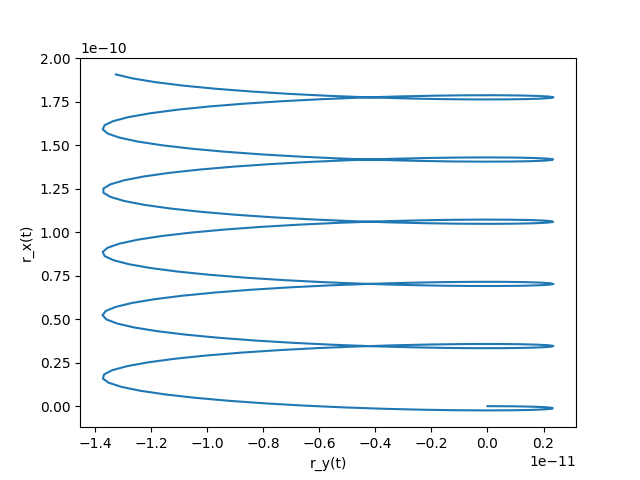
\includegraphics[width=\linewidth]{figures/no_rel_y_x.png}
	\caption{Gráfica $r_x(t)$ en función de $r_y(t)$}
	\label{fig:no_rel_y_x}
\end{figure}

\subsection{Discusión}

Las gráficas dejan claro que el ciclotrón tiene bien merecido su nombre, la partícula cargada, en este caso un electrón, acelerado en trayectoria de espiral, avanzando en dirección del eje-x.

La frecuencia angular ciclotrón es dada por:

$$
f = \frac{q}{m 2 \pi}B
$$

Por lo que $f \approx 3 \cdot 10^{10}$ y el periodo $T \approx 0.333 \cdot 10^{-10}$.

Vemos este periodo claramente presente en la figura \ref{fig:no_rel_x_y_z_t} para $\vec{r}_y(t)$ (la segunda fila). Es un poco menos evidente en la figura \ref{fig:no_rel_y_x}, pero si nos fijamos en el eje vertical (i.e: $\vec{r}_x(t)$) se puede percibir.

Si aproximamos la velocidad de deriva como: $\frac{\Delta \vec{r}_x(t)}{\Delta t}$, esto nos da: $v_{deriva} \approx \frac{2 \cdot 10^{-10}}{2 \cdot 10^{-10}} = 1$, que concuerda con el valor teórico dado por: $v_{deriva} = \frac{\vec{E} \times \vec{B}}{B^2} = (1, 0, 0)$. 
\newpage

\section{Ejercicio AR - Sistema de ED}

\subsection{Problema}

Utilizando coordenadas cartesianas en el espacio tridimensional para todas las magnitudes vectoriales, escriba el sistema de ecuaciones diferenciales pervio en términos de los componentes $x$, $y$, $z$ de $\vec{p}$, $\vec{v}$, $\vec{E}$ y $\vec{B}$.

La velocidad depende del momento a través de un factor $\gamma m$. Reescriba ese sistema de ecuaciones diferenciales en términos de los componentes del momento, dejando presente explícitamente el factor $\gamma m$.

\subsection{Resolución}

El sistema de ecuaciones dado por la fuerza de Lorentz es:

\begin{equation*}
\begin{bmatrix} 
	\diff{p_{rel_x}}{t} \\ \\
	\diff{p_{rel_y}}{t} \\ \\ 
	\diff{p_{rel_z}}{t} 
\end{bmatrix} = 
q \left( 
\begin{bmatrix} 
	E_x \\ E_y \\ E_z 
\end{bmatrix} + 
\begin{bmatrix} 
	v_x \\ v_y \\ v_z 
\end{bmatrix} 
	\times 
\begin{bmatrix} B_x \\ B_y \\ B_z \end{bmatrix} 
\right)
\end{equation*}

donde usamos $p_{rel}$ para ser explícito en que es el momento relativista.

La velocidad se puede reescribir en términos del momento: $ \vec{v} = \frac{1}{\gamma m} \vec{p}_{rel} $.

Por ende:

\begin{equation*}
	\begin{bmatrix} 
		\diff{p_{rel_x}}{t} \\ \\
		\diff{p_{rel_y}}{t} \\ \\ 
		\diff{p_{rel_z}}{t} 
	\end{bmatrix} = 
	q \left( 
	\begin{bmatrix} 
		E_x \\ E_y \\ E_z 
	\end{bmatrix} + 
\frac{1}{\gamma m}
	\begin{bmatrix} 
		p_{rel_x} \\ p_{rel_y} \\ p_{rel_z}
	\end{bmatrix} 
	\times 
	\begin{bmatrix} B_x \\ B_y \\ B_z \end{bmatrix} 
	\right) =
	\frac{q}{\gamma m} \left( 
(\gamma m)\begin{bmatrix} 
	E_x \\ E_y \\ E_z 
\end{bmatrix} + 
\begin{bmatrix} 
	p_{rel_x} \\ p_{rel_y} \\ p_{rel_z}
\end{bmatrix} 
\times 
\begin{bmatrix} B_x \\ B_y \\ B_z \end{bmatrix} 
\right)
\end{equation*}



\newpage

\section{Ejercicio BR - Factor Lorentz}

\subsection{Problema}
Exprese el valor del factor $\gamma m$ en términos de los componentes del momento. Finalmente, utilice esa expresión para reescribir el sistema de ecuaciones diferenciales en términos de los componentes cartesianos del momento e indique si se trata de un sistema de ecuaciones diferenciales acopladas o no.

\subsection{Resolución}

Empezamos por:

\begin{equation*}
	\gamma = 
\frac{1}{
	\sqrt{
	1 - \frac{|| \vec{v} ||^2} {c^2}	
}
}
\end{equation*}

podemos obtener una ecuación más fácil de manipular si:

\begin{align*}
	\gamma \sqrt{ 1 -  \frac{||\vec{v}||^2}{c^2}} &= 1 \\
	\gamma^2 (1 - \frac{||\vec{v}||^2}{c^2}) &= 1 \\
	\gamma ^2 - \frac{\gamma^2}{c^2} || \vec{v} ||^2 & =1
\end{align*}

Ahora reescribimos $||\vec{v}||^2$ en términos del momento relativista:

\begin{align*}
|| \vec{v} ||^2 
	&= \vec{v}\cdot \vec{v} \\
	&= \sum v_k^2 \\
	&= \sum (\frac{p_{rel_k}}{\gamma m})^2 \\
	&= \frac{1}{(\gamma m)^2} \sum p_{rel_k}^2 \\
\end{align*} 

Lo que finalmente da:

\begin{align*}
\gamma ^2 - \frac{\gamma^2}{c^2} || \vec{v} ||^2  &= 1 \\
\gamma ^2 - \frac{\gamma^2}{c^2} \frac{1}{(\gamma m)^2} \sum p_{rel_k}^2  &= 1
\end{align*}

Ahora podemos obtener una expresión para $\gamma m$:

\begin{align*} 
\gamma ^2 &=
1 + \frac{1}{(mc)^2} \sum p_{rel_k}^2 \\
m^2 \gamma^2 &= 
	m^2 + \frac{1}{c^2} \sum p_{rel_k} \\
m \gamma &=
	\sqrt{ 
	m^2 + \frac{1}{c^2} \sum p_{rel_k}	
}
\end{align*} 

Empezando por la última ecuación del ejercicio anterior:

\begin{equation*} 
\begin{bmatrix} 
	\diff{p_{rel_x}}{t} \\ \\
	\diff{p_{rel_y}}{t} \\ \\ 
	\diff{p_{rel_z}}{t} 
\end{bmatrix} = 
	\frac{q}{\gamma m} \left( 
(\gamma m)\begin{bmatrix} 
	E_x \\ E_y \\ E_z 
\end{bmatrix} + 
\begin{bmatrix} 
	p_{rel_x} \\ p_{rel_y} \\ p_{rel_z}
\end{bmatrix} 
\times 
\begin{bmatrix} B_x \\ B_y \\ B_z \end{bmatrix} 
\right)
\end{equation*} 

\begin{equation*} 
	\begin{bmatrix} 
		\diff{p_{rel_x}}{t} \\ \\
		\diff{p_{rel_y}}{t} \\ \\ 
		\diff{p_{rel_z}}{t} 
	\end{bmatrix} = 
	\frac{q}{\sqrt{ 
			m^2 + \frac{1}{c^2} \sum p_{rel_k}	
	}} \left( 
	(\sqrt{ 
		m^2 + \frac{1}{c^2} \sum p_{rel_k}	
	})\begin{bmatrix} 
		E_x \\ E_y \\ E_z 
	\end{bmatrix} + 
	\begin{bmatrix} 
		p_{rel_x} \\ p_{rel_y} \\ p_{rel_z}
	\end{bmatrix} 
	\times 
	\begin{bmatrix} B_x \\ B_y \\ B_z \end{bmatrix} 
	\right)
\end{equation*} 

Evidentemente estamos ante un sistema de ecuaciones diferenciales acopladas, ya que la ecuación diferencial de cada componente del momento depende de los otros componentes. Esto no sólo es debido a $\gamma$ sino también por $\vec{p}_{rel} \times \vec{B}$ (en el caso de $\vec{B}$ no nulo).
\newpage

\section{Ejercicio CR - Momento Lineal}

\subsection{Problema}
Escriba el sistema de ecuaciones diferenciales que describe la posición de la partícula en términos de los componentes del momento lineal.

\subsection{Resolución}

Dado que:

$$
\diff{\vec{r}(t)}{t} = \vec{v}(t) = \frac{1}{\gamma m} \vec{p}_{rel}(t)
$$

Obtenemos el sistema de ecuaciones diferenciales:

\begin{equation*} 
	\begin{bmatrix} 
		\diff{r_x}{t} \\ \\
		\diff{r_y}{t} \\ \\ 
		\diff{r_z}{t} 
	\end{bmatrix} = 
\frac{1}{\gamma m}
\begin{bmatrix}
	p_{rel_x}(t) \\ \\ p_{rel_y}(t) \\ \\ p_{rel_z}(t)
\end{bmatrix}
\end{equation*} 
y: 

\begin{equation*} 
	\begin{bmatrix} 
		\diff{r_x}{t} \\ \\
		\diff{r_y}{t} \\ \\ 
		\diff{r_z}{t} 
	\end{bmatrix} = 
	\frac{1}{\sqrt{ 
			m^2 + \frac{1}{c^2} \sum p_{rel_k}	
	}}
	\begin{bmatrix}
		p_{rel_x}(t) \\ \\ p_{rel_y}(t) \\ \\ p_{rel_z}(t)
	\end{bmatrix}
\end{equation*} 

\newpage

\section{Ejercicio DR - Sistema de ED Completo}

\subsection{Problema}
Presente el sistema de ecuaciones diferenciales completo que hay que resolver para describir el movimiento de una partícula cargada bajo la acción simultánea de un campo eléctrico y magnético. ¿Cuántas ecuaciones diferenciales de primer orden es preciso resolver?

\subsection{Resolución}

El sistema completo consiste en las siguientes ecuaciones:

\begin{equation*} 
	\begin{bmatrix} 
	\diff{r_x}{t} \\ \\
	\diff{r_y}{t} \\ \\ 
	\diff{r_z}{t} \\ \\
	\diff{p_{rel_x}}{t} \\ \\
	\diff{p_{rel_y}}{t} \\ \\ 
	\diff{p_{rel_z}}{t} 
\end{bmatrix} = 
\begin{bmatrix}
	p_{rel_x}(t) \\ \\ p_{rel_y}(t) \\ \\ p_{rel_z}(t)
\\ \\
		\frac{q}{\sqrt{ 
			m^2 + \frac{1}{c^2} \sum p_{rel_k}	
	}} \left( 
	(\sqrt{ 
		m^2 + \frac{1}{c^2} \sum p_{rel_k}	
	})\begin{bmatrix} 
		E_x \\ E_y \\ E_z 
	\end{bmatrix} + 
	\begin{bmatrix} 
		p_{rel_x} \\ p_{rel_y} \\ p_{rel_z}
	\end{bmatrix} 
	\times 
	\begin{bmatrix} B_x \\ B_y \\ B_z \end{bmatrix} 
	\right)
\end{bmatrix} 
\end{equation*}

En total 6 ecuaciones de primer orden.
\newpage

\section{Ejercicio ER - Sistema de ED Completo}

\subsection{Problema}

Utilizando un Runge-Kutta de cuarto orden con un paso temporal de $\Delta t = 10^{-12} s$ realice la simulación necesaria para describir el movimiento del electrón cuando parte de las condiciones iniciales

\begin{align*}
	\vec{r}(0) &= \gamma m c  (-1, 1, 0 )\ \text{m} \\
	\vec{v}(0) &= \frac{2c}{3} 
		(
			\sin \frac{\pi}{9},
			0,
			\cos \frac{\pi}{9} 
		) \ \text{m\slash s}
\end{align*} 

hasta un tiempo total $t = 200\ \text{ns}$. Indique los resultados obtenidos para todas las magnitudes (posiciones y momentos de la partícula) calculadas con el Runge-Kutta en las dos primeras iteraciones temporales.

\subsection{Resolución} 

El código que resuelve este ejercicio se puede ver en \ref{code:ex10}.

Los resultados completos se pueden ver en el repositorio git y los primeros 50 puntos están en \ref{data:r_v_rel}. 

Los valores para las dos iteraciones temporales son:

\begin{table}[H]
	\centering
	\csvreader[
	tabular=|c|l|l|l|,
	table head=\hline \textbf{t} & \textbf{$r_x$} & \textbf{$r_y$} & \textbf{$r_z$} \\\hline,
	filter test=\ifnumless{\thecsvrow}{3},
	late after last line=\\\hline,
	]{data/simul_rel_r_capped.csv}{}{\csvlinetotablerow}
\end{table}

\begin{table}[H]
	\centering
	\csvreader[
	tabular=|c|l|l|l|,
	table head=\hline \textbf{t} & \textbf{$v_x$} & \textbf{$v_y$} & \textbf{$v_z$} \\ \hline,
	filter test=\ifnumless{\thecsvrow}{3},
	late after last line=\\\hline,
	]{data/simul_rel_v_capped.csv}{}{\csvlinetotablerow}
\end{table}



\newpage

\section{Ejercicio FR - Gráficas}

\subsection{Problema}

Represente la trayectoria de la partícula en el espacio tridimensional y analice los resultados.

Presente en una misma gráfica el comportamiento de tres velocidades adimensionales (extraídas de la anterior simulación) en función del tiempo medido en nanosegundos. En concreto, se pide el módulo de la velocidad del electrón relativista en función del tiempo, el componente $v_z$ de su velocidad y su velocidad radial $v_r = \sqrt{ v_x^2 + v_y^2}$. 

\subsection{Resolución}

El código que resuelve este ejercicio se puede ver en \ref{code:ex11}.

\paragraph{Gráfica de $\vec{r}(t)$} 
Primero mostramos los componentes de $\vec{r}(t)$ en función de $t$.

\begin{figure}[H]
	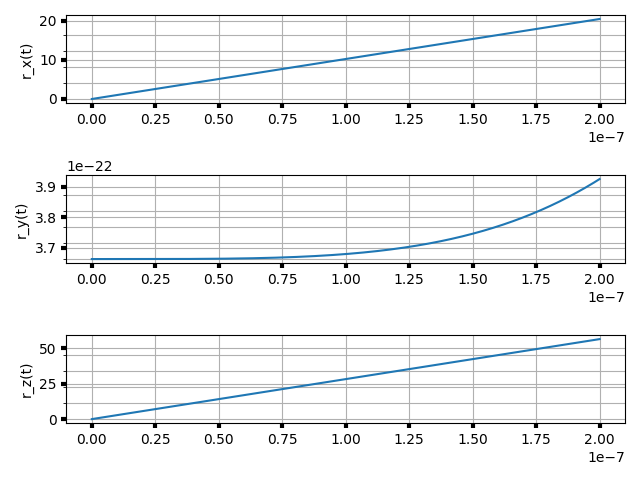
\includegraphics[width=\linewidth]{figures/rel_rx_ry_rz.png}
	\caption{Gráfica $r_x(t)$, $r_y(t)$, $r_z(t)$ en función de $t$}
	\label{fig:rel_rx_ry_rz_t}
\end{figure}

\newpage 

\paragraph{Gráfica en 3D de $\vec{r}(t)$} 
La trayectoria de la partícula en 3D.

\begin{figure}[H]
	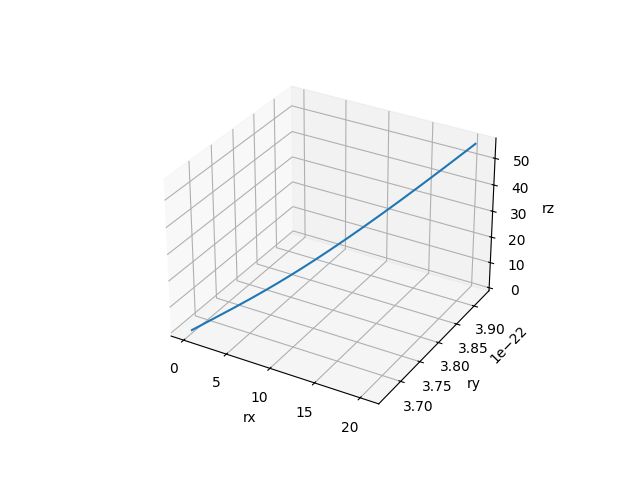
\includegraphics[width=\linewidth]{figures/rel_3d_r.png}
	\caption{Gráfica $r_x(t)$, $r_y(t)$, $r_z(t)$ en 3D}
	\label{fig:rel_3d_r}
\end{figure}

\newpage 

\paragraph{Gráfica de $\frac{\vec{v}(t)}{c}$}

La gráfica de los componentes de $\vec{v}(t)$ adimensionada por $c$.

\begin{figure}[H]
	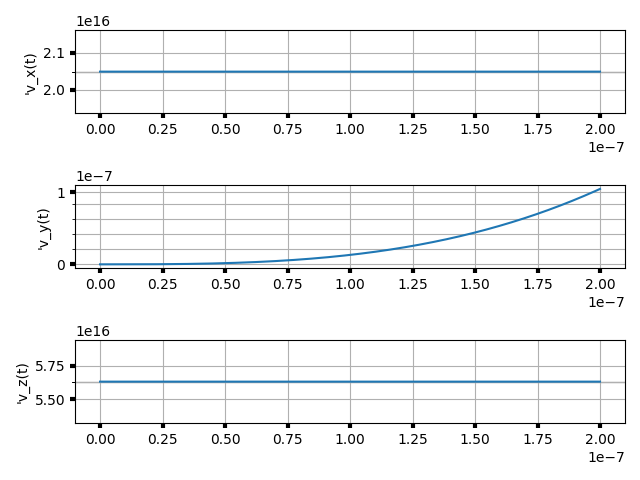
\includegraphics[width=\linewidth]{figures/rel_adim_vx_vy_vz.png}
	\caption{Gráfica $\vec{v}(t)$ adimensionada}
	\label{fig:rel_adim_vx_vy_vz}
\end{figure}

\newpage 

\paragraph{Gráfica de $||v||, v_{radial}$ y $v_z$} La gráfica de $||v||$, $v_r$ y $v_z$ (adimensionadas por $c$).

\begin{figure}[H]
	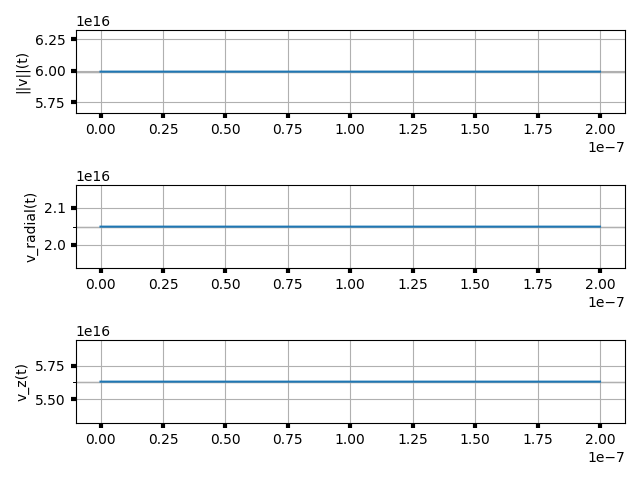
\includegraphics[width=\linewidth]{figures/rel_v_mod_rad_z.png}
	\caption{Gráfica $v_r$ y $v_z$}
	\label{fig:rel_v_radial_vz}
\end{figure}

\newpage

\section{Ejercicio GR - Conclusiones}

\subsection{Problema}

Extraiga las conclusiones de todos los resultados del trabajo (parte no relativista y relativista).


\subsection{Discusión sobre la realización del trabajo}

Quizás lo que más me ha sorprendido de este trabajo, y que consecuentemente ha sido de gran aprendizaje, es lo potente que es combinar el método RK4 con la capacidad de procesado de datos que aporta el PC. 


\paragraph{Posibles errores}
En las dos partes, lo más complicado ha sido hacer a mano los cálculos para expresar el problema como un sistema de ecuaciones diferenciales de primer orden, teniendo mucho cuidado con los signos y demás detalles (e.g: el haberme equivocado y escrito un '+' donde tenía que haber un '-' significó pasarme unas horas buscando un bug cuando el error no estaba en el código...).

También se me hizo muy claro la utilidad de hacer tests sobre el algoritmo, para asegurarme que la implementación del método fue correcta (e.g: para asegurarme que implementé el algoritmo RK4 de forma correcta hice algunos tests donde $\vec{y}(t) = [\sin wt, \cos wt]$, y comprobé los resultados de una simulación con los valores teóricos). Esto ayuda muchísimo cuando estás generando datos incorrectos y tienes que ver si los errores están en el algoritmo, en el sistema calculado a mano, o en el traspaso del sistema de papel a código.

\paragraph{Visualización e interpretación}

Noté lo díficil que puede llegar ser extraer una interpretación de los datos, pues simular es sólo una parte del problema, luego hay que visualizar e interpretar los resultados.  

\subsection{Discusión sobre los resultados}

\subsubsection{Parte no relativista} En la parte no relativista, hicimos una simulación de un ciclotrón, donde los resultados mostraban a la partícula haciendo una trayectoria de espiral, avanzando principalmente en la dirección del eje-x. 

\subsubsection{Parte relativista} Aquí, al visualizar el módulo de la velocidad, así como la velocidad radial y del componente $v_z$, se puede ver que son valores constantes. Cosa poco sorprendente pues no hay campo $E$ y el campo $B$ es no-uniforme pero estático, por ende no hace trabajo sobre la partícula.  

\paragraph{Error numérico}No me he puesto a hacer cálculos para comprobar esto, pero es muy posible que los valores de los componentes $r_y$ y $v_y$ sean producto de un error numérico, dada la descomunal diferencia en el orden de magnitud entre el componente-y con los componentes x y z de la velocidad y la posición. Quizás modificando el algoritmo para usar sumas compensadas (e.g: Kahan) minimice la presencia de estos errores (aunque hay más fuentes de errores). 

\newpage

% apendice
\section{Apéndice}

\subsection{Código linalg}
\label{code:linalg}

\lstinputlisting[language=Python]{../../code/methods/linalg.py}


\subsection{Código datos}
\label{code:datos}

\lstinputlisting[language=Python]{../../code/pecs/pec4/data.py}

\subsection{Código Ejercicio C}
\label{code:ex3}

\lstinputlisting[language=Python]{../../code/pecs/pec4/ex3.py}

\subsection{Código Ejercicio D}
\label{code:ex4}

\lstinputlisting[language=Python]{../../code/pecs/pec4/ex4.py}

\subsection{Código Ejercicio E}
\label{code:ex5}

\lstinputlisting[language=Python]{../../code/pecs/pec4/ex5.py}

\subsection{Código Ejercicio F}
\label{code:ex6}

\lstinputlisting[language=Python]{../../code/pecs/pec4/ex6.py}

\subsection{Código Ejercicio G}
\label{code:ex7}

\lstinputlisting[language=Python]{../../code/pecs/pec4/ex7.py}
\newpage



\end{document}
